\documentclass[proposal]{cmpreport}
\graphicspath{ {./images/} }

\title{GPU Accelerated Method for Constructing and Rendering Trees 
        \\ - \\ 
        Project Proposal First Draft}
\author{Thomas Mcloughlin}
\date{02/10/2020}
\registration{100203952}
\ccode{CMP - 6013Y}
\supervisor{Dr. Stephen Laycock}

\begin{document}
\maketitle

\pagebreak
\section{Introduction}
Generating natural environments can be costly. Creating and rendering realistic 
models of trees can be challenging. The aim of this project is to investigate 
approaches for creating and rendering trees to be used in a real-time graphics 
application.

\section{Description of Project}

\subsection{Aims}
The aim of this project is to create an OpenGL module for constructing and rendering 
trees for use in 3D environments such as games. The trees that are constructed should 
look relatively realistic and the rendering process should make effective use of the 
GPU to be as efficient as possible.

\subsection{Motivation}
The motivation for creating this project is to make the addition of trees into a 3D 
environment easier to allow for the creation of better looking environments without 
needing to spend as much time modeling certain assets. \\
The natural growth patterns of trees can be represented quite well algorithmically so 
I would argue that using an algorithm to produce tree models will also result in a 
more realistic looking model than one created manually while taking less time and 
effort.

\subsection{Understanding of Issues and Problems}
The issues and problems that this project would aim to solve would revolve mainly 
around the difficulties of producing realistic looking trees manually and then having 
to insert them into your scene. \\

The user could choose to either make their own trees or acquire premade assets:
\begin{itemize}
        \item If they decide to produce their own trees it would take a long time to 
              model a realistic tree and it is also very hard to make a realistic 
              looking model.
        \item If they decide to use premade assets it may cost money to acquire decent 
              assets and it might not be possible to find the kind of specific tree they 
              want. 
\end{itemize}

My solution would help solve these problems by allowing an automatic construction 
for the trees to avoid any modeling by the user and by including modifiable parameters 
the user can tweak, they could produce whatever tree they want for their scene.

\pagebreak
\section{Market Analysis}
As part of analysing this project I have researched some similar software solutions 
that are already available on the market.

\subsection{SpeedTree 3D Vegetation Modeling}
SpeedTree \cite{speedtree} is an advanced software suite that is used for large projects 
in the game and film industry. It allows for extremely detailed foliage generation, 
not limited to trees, and allows for very minute detail manipulation for the generated 
plants. This includes factors such as tree bark colour and texture, and the size, shape 
and scattering of leaves across branches.

\subsection{The Grove 3D Tree Growing Software}
The Grove \cite{thegrove} is a detailed simulated method of constructing trees with a 
multitude of factors that come into play with the growth of the tree. The Grove uses a 
different method than might be assumed for typical construction of trees. Rather than 
construct trees in one state, by that I mean that you construct the tree as you would 
want to display it, The Grove gives you a set of many parameters that you can tweak and 
you then grow a tree, by adding years to its life and tweaking the parameters you 
construct the tree you want. This includes modifying the weight of branches, the flow 
of sugar and hormones within the tree, growing towards light sources, growing around 
or avoiding buildings and many others.

\pagebreak
\section{Method Analysis}
I have also researched some existing methods used to construct trees and how they 
relate to the scope of this project. I have also included research into general 
GPU accelerated rendering as I believe that will also be useful information.

\subsection{Modeling Trees with a Space Colonization Algorithm}
The paper \cite{colonization} is a wealth of knowledge on the construction of trees. 
It includes a well written and explained method for constructing trees and provides 
many links to other relevant papers that relate to various aspects of the tree 
construction. The main method they describe involves creating a three-dimensional 
\textit{envelope} of the tree crown that you want to produce. You then give a set of 
\textit{attraction points} which the paper states as user inputted but I think could be 
randomly generated using a noise algorithm. The tree \textit{skeleton} then grows, from a 
given root point, into the envelope and towards the attraction points which produces 
branches within the given space. Once the skeleton is produced it can be used as a 
base to apply thickness to the trunk and branches.

\begin{figure}[h]
        \caption{Key steps of the proposed method}
        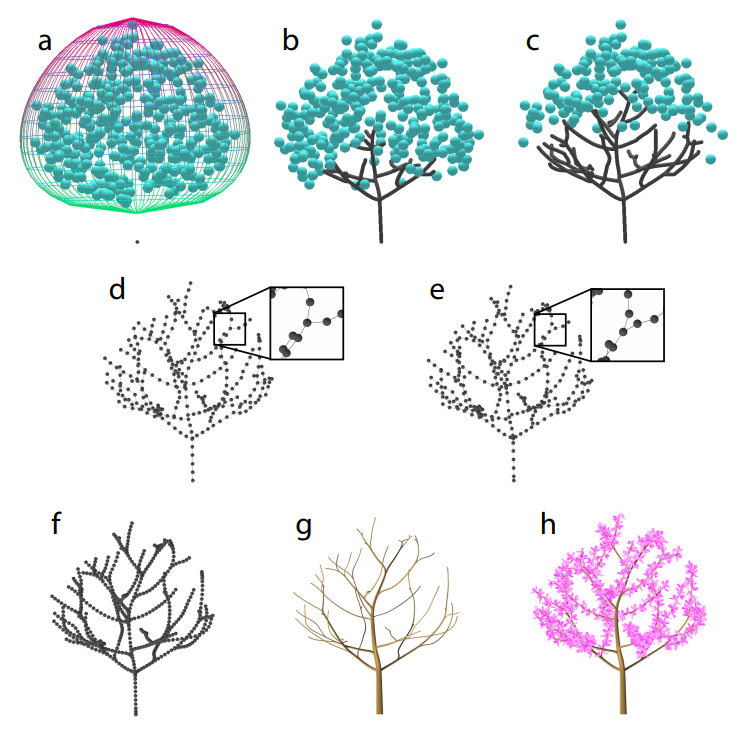
\includegraphics[scale=0.47]{AttractionPoints}
        \centering
\end{figure}

This is a very basic overview of course and I will research further into this method 
once I am sure of the scope and aim of the project. Whether I use this method or not 
however, I believe that this paper and it's references will be of great use moving 
forward.

\subsection{The Algorithmic Beauty of Plants}
This book \cite{beautyOfPlants} provides many insights into the algorithmic construction 
of plants. After a brief look through it seems that the most relevant section will be 
chapter 2 "Modeling of trees" which puts forward a method of generating branches through 
a \textit{mother branch} having two \textit{daughter branches} that split off from it. 
These daughter branches are shortened using constant ratios with repect to the mother 
branch and are angled from the mother branch using constant \textit{branching angles}. 
The mother branch and daughter branches are contained in the same \textit{branch plane}.

\begin{figure}[h]
        \caption{Proposed tree geometry}
        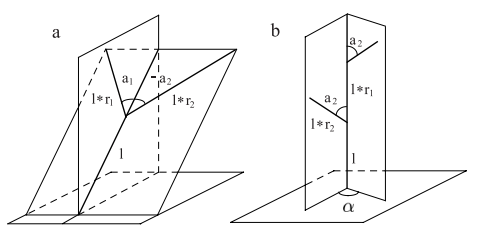
\includegraphics{MDbranches}
        \centering
\end{figure}

This book was co-authored by Przemysław Prusinkiewicz who was also a co-author of the 
space colonization paper I referenced previously. It seems that his research into 
the 3D construction of plants will be useful while researching for this project. 
Once I am sure of the direction I'm taking the project I will read into this book more 
closely to glean more details that could aid my progress.

\pagebreak
\section{Proposed Approaches}

\pagebreak
\section{Risks}

\pagebreak
\bibliography{bibfile}
\end{document}